%%%%%%%%%%%%%%%%%%%%%%%%%%%%%%%%%%%%%%%%%
% Beamer Presentation
% LaTeX Template
% Version 1.0 (10/11/12)
%
% This template has been downloaded from:
% http://www.LaTeXTemplates.com
%
% License:
% CC BY-NC-SA 3.0 (http://creativecommons.org/licenses/by-nc-sa/3.0/)
%
%%%%%%%%%%%%%%%%%%%%%%%%%%%%%%%%%%%%%%%%%

%----------------------------------------------------------------------------------------
%	PACKAGES AND THEMES
%----------------------------------------------------------------------------------------

\documentclass[mathserif]{beamer}

\mode<presentation> {

% The Beamer class comes with a number of default slide themes
% which change the colors and layouts of slides. Below this is a list
% of all the themes, uncomment each in turn to see what they look like.

%\usetheme{default}
%\usetheme{AnnArbor}
\usetheme{Antibes} %++
%\usetheme{Bergen}
%\usetheme{Berkeley}
%\usetheme{Berlin}
%\usetheme{Boadilla}
%\usetheme{CambridgeUS} %+
%\usetheme{Copenhagen}
%\usetheme{Darmstadt} %++
%\usetheme{Dresden}
%\usetheme{Frankfurt}
%\usetheme{Goettingen}
%\usetheme{Hannover}
%\usetheme{Ilmenau} %++
%\usetheme{JuanLesPins}
%\usetheme{Luebeck}
%\usetheme{Madrid}
%\usetheme{Malmoe}
%\usetheme{Marburg}
%\usetheme{Montpellier}
%\usetheme{PaloAlto}
%\usetheme{Pittsburgh}
%\usetheme{Rochester}
%\usetheme{Singapore}
%\usetheme{Szeged}
%\usetheme{Warsaw}

% As well as themes, the Beamer class has a number of color themes
% for any slide theme. Uncomment each of these in turn to see how it
% changes the colors of your current slide theme.

%\usecolortheme{albatross}
\usecolortheme{beaver}
%\usecolortheme{beetle}
%\usecolortheme{crane}
%\usecolortheme{dolphin}
%\usecolortheme{dove}
%\usecolortheme{fly}
%\usecolortheme{lily}
%\usecolortheme{orchid}
%\usecolortheme{rose}
%\usecolortheme{seagull}
%\usecolortheme{seahorse}
%\usecolortheme{whale}
%\usecolortheme{wolverine}

%\setbeamertemplate{footline} % To remove the footer line in all slides uncomment this line
\setbeamertemplate{footline}[frame number] % To replace the footer line in all slides with a simple slide count uncomment this line

\setbeamertemplate{navigation symbols}{} % To remove the navigation symbols from the bottom of all slides uncomment this line
}

\usepackage{graphicx} % Allows including images
\usepackage{booktabs} % Allows the use of \toprule, \midrule and \bottomrule in tables
\usepackage[utf8x]{inputenc}
\usepackage[spanish]{babel}
\usepackage{tikz,times}
\usepackage{multicol}
\usepackage{verbatim}
\usetikzlibrary{mindmap,trees,backgrounds}

  % Keys to support piece-wise uncovering of elements in TikZ pictures:
  % \node[visible on=<2->](foo){Foo}
  % \node[visible on=<{2,4}>](bar){Bar}   % put braces around comma expressions
  %
  % Internally works by setting opacity=0 when invisible, which has the 
  % adavantage (compared to \node<2->(foo){Foo} that the node is always there, hence
  % always consumes space plus that coordinate (foo) is always available.
  %
  % The actual command that implements the invisibility can be overriden
  % by altering the style invisible. For instance \tikzsset{invisible/.style={opacity=0.2}}
  % would dim the "invisible" parts. Alternatively, the color might be set to white, if the
  % output driver does not support transparencies (e.g., PS) 
  %
\tikzset{
    invisible/.style={opacity=0},
    visible on/.style={alt={#1{}{invisible}}},
    alt/.code args={<#1>#2#3}{%
      \alt<#1>{\pgfkeysalso{#2}}{\pgfkeysalso{#3}} % \pgfkeysalso doesn't change the path
    },
  }

%----------------------------------------------------------------------------------------
%	TITLE PAGE
%----------------------------------------------------------------------------------------

\title[Evaluación de modelos de aprendizaje automático
para posicionamiento indoor utilizando Bluetooth
low energy]{Evaluación de modelos de aprendizaje automático
para posicionamiento indoor utilizando Bluetooth
low energy\\\normalsize Trabajo de Memoria} % The short title appears at the bottom of every slide, the full title is only on the title page

\author{Felipe Berrios Toloza} % Your name
\institute[UTFSM] % Your institution as it will appear on the bottom of every slide, may be shorthand to save space
{
Universidad Técnica Federico Santa María \\ % Your institution for the title page
\medskip
\textit{felipe.berriost@alumnos.usm.cl} % Your email address
}
\date{11 de abril de 2018} % Date, can be changed to a custom date

\begin{document}

\begin{frame}
\titlepage % Print the title page as the first slide
\end{frame}

\begin{frame}{Tabla de Contenidos}
\begin{multicols}{2}
  \tableofcontents
\end{multicols}
\end{frame}


\AtBeginSection[]
{
  \begin{frame}{Tabla de Contenidos}
   \begin{multicols}{2}
     \tableofcontents[currentsection,hideothersubsections]
   \end{multicols}
  \end{frame}
}

%----------------------------------------------------------------------------------------
%	PRESENTATION SLIDES
%----------------------------------------------------------------------------------------

%------------------------------------------------
\section{Introducción} 
%------------------------------------------------

\begin{frame}
\frametitle{Introducción}

\textbf{Geolocalización}
\begin{itemize}

%\item La geolocalización ha jugado un papel fundamental en las últimas décadas.

\item Usado ampliamente por el sector militar, académico e industrial.

\item Cada vez se vuelve más accesible: basta con tener un smartphone o similar para poder geolocalizarse.

\begin{itemize}
\item 2 mil millones de \textit{smartphones} activos en el mundo\footnote{Worldwide Internet and Mobile Users, eMarketer, 2015.}.
\end{itemize}

\end{itemize}



\end{frame}


%------------------------------------------------
\subsection{Descripción del Problema}

\begin{frame}
\frametitle{Descripción del Problema}

\begin{itemize}

\item Alta demanda en el posicionamiento en interiores
\pause
\item Tecnologías de geolocalización satelital como GPS funciona de manera limitada o nula en ambientes interiores

\end{itemize}

\pause
\vspace*{.5cm}
\textbf{¿Cómo podemos conocer nuestra posición en dichos lugares? }




\end{frame}

%------------------------------------------------

\subsection{Objetivos} % A subsection can be created just before a set of slides with a common theme to further break down your presentation into chunks

\begin{frame}
\frametitle{Objetivos}

\begin{itemize}
\item Identificar los métodos y tecnologías que actualmente permiten conocer la posición.
\pause
\item Determinar los \textit{trade-offs} entre exactitud y costo para tecnologías de posicionamiento \textit{indoor}
\end{itemize}

\end{frame}

%------------------------------------------------
\section{Estado del Arte}
%------------------------------------------------

\subsection{Métodos de Posicionamiento}
\begin{frame}
\frametitle{Métodos de Posicionamiento}

%  MAPA MENTAL DE MATERIALES
\centering
\resizebox{!}{0.6\textwidth}{%
\begin{tikzpicture}
  \path[mindmap,concept color=gray!30!,text=red!60!black]
    node[concept] {Métodos de posicionamiento}
    [clockwise from=0]
    child[visible on=<5->,concept color=gray!30!,text=red!60!black] { node[concept] {Trilateración} }  
    child[visible on=<4->,concept color=gray!30!,text=red!60!black] { node[concept] {Triangulación} }
    child[visible on=<3->,concept color=gray!30!,text=red!60!black] { node[concept] {Basado en celdas de origen} }
    child[visible on=<2->,concept color=gray!30!,text=red!60!black] { node[concept] {\textit{Fingerprints}} };
\end{tikzpicture}
}
\end{frame}

%------------------------------------------------

\begin{frame}
\frametitle{Fingerprints}

\begin{figure}
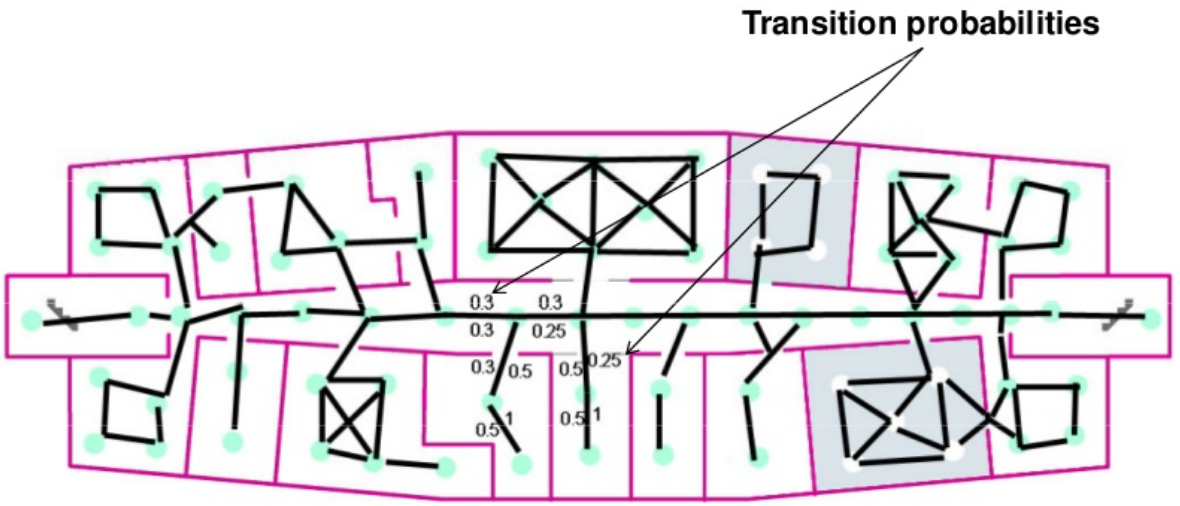
\includegraphics[width=\linewidth]{../figures_chesta/estado_del_arte/fingerprints}
\end{figure}

\end{frame}

%------------------------------------------------

\begin{frame}
\frametitle{Basado en celdas de origen}

\begin{figure}
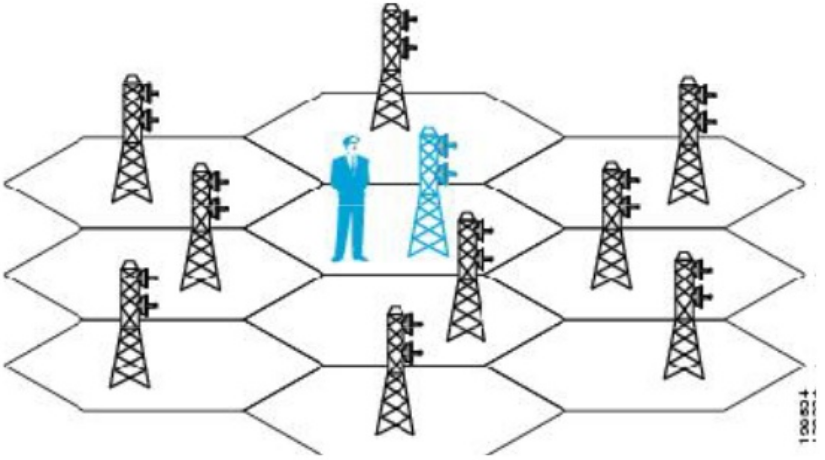
\includegraphics[width=.8\linewidth]{../figures_chesta/estado_del_arte/conection_based_positioning}
\end{figure}

\end{frame}

%------------------------------------------------

\begin{frame}
\frametitle{Triangulación}

\begin{figure}
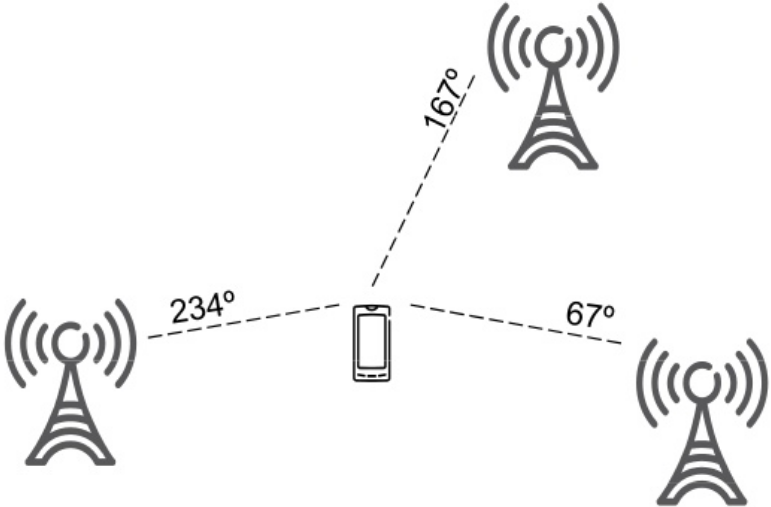
\includegraphics[width=.8\linewidth]{../figures_chesta/estado_del_arte/triangulation}
\end{figure}

\end{frame}

%------------------------------------------------

\begin{frame}
\frametitle{Trilateración}

\begin{figure}
\includegraphics[width=.7\textheight]{../figures_chesta/estado_del_arte/trilateration}
\end{figure}

\end{frame}

%------------------------------------------------


\begin{frame}
\frametitle{Trilateración}

\begin{columns}[t] % The "c" option specifies centered vertical alignment while the "t" option is used for top vertical alignment

\column{.5\textwidth} % Left column and width

\visible<1->{$P_1$, $P_2$, $P_3$, $r_1$, $r_2$ y $r_3$ conocidos}
\visible<2->{¿Cuál es la posición de $B$?}

\vspace*{.15\textwidth}

\visible<3->{\begin{equation*}
x^2+y^2+z^2=r_1^2
\end{equation*}
\begin{equation*}
(x-d)^2+y^2+z^2=r_2^2
\end{equation*}
\begin{equation*}
(x-i)^2+(y-j)^2+z^2=r_3^2
\end{equation*}
}
\column{.5\textwidth} % Right column and width
\begin{figure}
\includegraphics[width=\textwidth]{../figures_chesta/estado_del_arte/trilateration}
\end{figure}

\end{columns}

\end{frame}

%------------------------------------------------

\begin{frame}
\frametitle{Trilateración}

\begin{columns}[t] % The "c" option specifies centered vertical alignment while the "t" option is used for top vertical alignment

\column{.5\textwidth} % Left column and width

$P_1$, $P_2$, $P_3$, $r_1$, $r_2$ y $r_3$ conocidos
¿Cuál es la posición de $B$?

\vspace*{.1\textwidth}

\begin{equation*}
x=\frac{r_1^2-r_2^2-d^2}{2d}
\end{equation*}
\begin{equation*}
y=\frac{r_1^2-r_3^2-x^2+i^2+j^2}{2j}-\frac{i}{j}x
\end{equation*}
\begin{equation*}
z=\pm\sqrt{r_1^2-x^2-y^2}
\end{equation*}

\column{.5\textwidth} % Right column and width
\begin{figure}
\includegraphics[width=\textwidth]{../figures_chesta/estado_del_arte/trilateration}
\end{figure}

\end{columns}

\end{frame}

%------------------------------------------------

\subsection{Tecnologías que permiten la geolocalización}

\begin{frame}
\frametitle{Tecnologías que permiten la geolocalización}

\begin{columns}[t]

\column{.5\textwidth}
\textbf{Posicionamiento \textit{outdoor}}

\begin{itemize}
\item Sistemas satelitales (GPS, GLONASS, Galileo, Beidou)
\item Localización por antenas móviles (GSM)
\end{itemize}


\column{.5\textwidth}
\textbf{Posicionamiento \textit{indoor} (IPS)}

\begin{itemize}
\item Wi-Fi
\item Bluetooth
\item RFID
%\item Magnetismo
\end{itemize}

\end{columns}

\end{frame}

%------------------------------------------------

\begin{frame}
\frametitle{Posicionamiento \textit{outdoor}}

\begin{columns}[t]

\column{.5\textwidth}

\textbf{GPS}

\begin{itemize}
\item Red de 24 satélites 
\item Precisión del orden de centímetros a unos pocos metros
\item Requiere línea de visión directa (\textit{Line of Sight})
\end{itemize}

\column{.55\textwidth}

\textbf{GSM}

\begin{itemize}
\item Localización principalmente por Celdas de Origen y triangulación
\item Precisión del orden de 50m a 4km
\item Menor gasto energético
\end{itemize}



\end{columns}
\end{frame}

%------------------------------------------------

\begin{frame}
\frametitle{Posicionamiento \textit{indoor} - WiFi}

\begin{block}{Free-space path loss (FSPL)}
FSPL es la pérdida de la intensidad de señal que ocurre cuando una onda electromagnética viaja desde un transmisor a un receptor a través de una línea de visión directa en un espacio libre.	
\end{block}

\begin{figure}
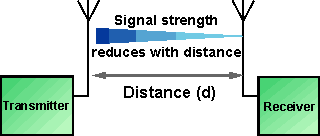
\includegraphics[width=.65\textwidth]{../figures_chesta/estado_del_arte/fspl}
\end{figure}

\end{frame}

%------------------------------------------------
\begin{frame}
\frametitle{Posicionamiento \textit{indoor} - WiFi}

\begin{columns}

\column{.60\textwidth}

\begin{equation*}
FSPL=\Bigg(\frac{4\pi df}{c}\Bigg)^2
\end{equation*}

\begin{equation*}
FSPL(dB)=20 log(d)+20 log(f) + K
\end{equation*}

\begin{equation*}
d=10^{\frac{1}{20}(K-20 log(f)+FSPL)}
%d=10^{\frac{K-20 log(f)+FSPL}{20}}
\end{equation*}

\column{.5\textwidth}

\begin{figure}
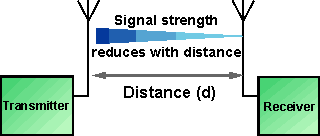
\includegraphics[width=\textwidth]{../figures_chesta/estado_del_arte/fspl}
\end{figure}

\end{columns}

\end{frame}

%------------------------------------------------

\begin{frame}
\frametitle{Posicionamiento \textit{indoor} - Bluetooth}

\begin{itemize}
\item Bluetooth 4.0 (\textit{Bluetooth Low Energy})
\item Beacons
\end{itemize}

\begin{figure}
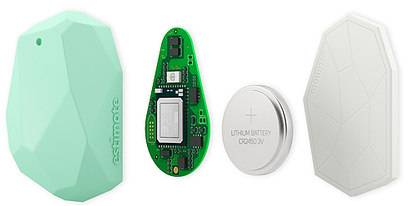
\includegraphics[width=.5\textwidth]{../figures_chesta/estado_del_arte/beacons_estimote}
\end{figure}

\end{frame}

%------------------------------------------------

\begin{frame}
\frametitle{Posicionamiento \textit{indoor} - Bluetooth}

\begin{block}{Tx Power}
Potencia constante transmitida por cada Beacon. A medida que la señal se aleja del beacon va decayendo su valor.
\end{block}

\begin{block}{RSSI}
Escala de referencia para medir el nivel de potencia de las señales recibidas por un dispositivo.  
\end{block}



\begin{equation*}
d = 0,899\Bigg(\frac{RSSI}{TxPower}\Bigg)^{7,771}+0,111
\end{equation*}



\end{frame}

%------------------------------------------------

\begin{frame}
\frametitle{Posicionamiento \textit{indoor} - RFID}

\begin{columns}[c]

\column{.5\textwidth}

\begin{itemize}

\item Posee tres componentes
\begin{enumerate}[1]
\item Lector de etiquetas
\item Ordenador central
\item Transpondedor
\end{enumerate}

\visible<2->{
\item Posicionamiento basado en celdas de origen}

\end{itemize}

 


\column{.5\textwidth}

\begin{figure}
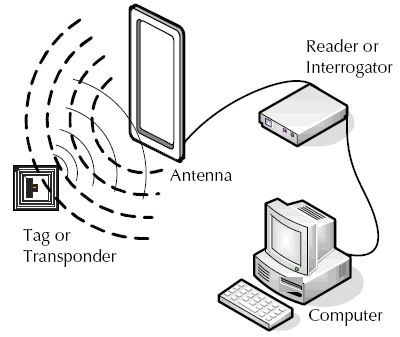
\includegraphics[width=\textwidth]{../figures_chesta/estado_del_arte/how_rfid_works}
\end{figure}

\end{columns}


\end{frame}

%------------------------------------------------

\begin{comment}

\begin{frame}
\frametitle{Posicionamiento \textit{indoor} - Magnetismo}

\begin{itemize}
\item Cada pieza de metal dentro de un edificio interfiere de manera única con el campo magnético de la Tierra
\item No requiere la instalación de componentes físicos extras
\item Es necesario mapear el edificio completo
\end{itemize}


\end{frame}

\end{comment}

%------------------------------------------------
\section{Diseño del Estudio}
%------------------------------------------------
\subsection{Cualidades y costos de tecnologías}
\begin{frame}
\frametitle{Cualidades y costos de tecnologías - WiFi}

\vspace*{-1cm}
\begin{table}[H]
\centering
\label{tab:rango_wifi}
\resizebox{\textwidth}{!}{
\begin{tabular}{|c|c|c|c|c|}
\hline
\begin{tabular}[c]{@{}c@{}}\textbf{Protocolo} \\ \textbf{802.11}\end{tabular} & \begin{tabular}[c]{@{}c@{}}\textbf{Frecuencia}\\ \textbf{{[}GHz{]}}\end{tabular} & \begin{tabular}[c]{@{}c@{}}\textbf{Banda ancha}\\ \textbf{{[}MHz{]}}\end{tabular} & \begin{tabular}[c]{@{}c@{}}\textbf{Rango indoor} \\ \textbf{aproximado {[}m{]}}\end{tabular} & \begin{tabular}[c]{@{}c@{}}\textbf{Rango outdoor}\\\textbf{ aproximado {[}m{]}}\end{tabular} \\ \hline \hline
a                                                           & 3.7/ 5                                                         & 20                                                              & 35                                                                         & 120                                                                        \\ \hline
b                                                           & 2.4                                                            & 20                                                              & 35                                                                         & 140                                                                        \\ \hline
g                                                           & 2.4                                                            & 20                                                              & 50                                                                         & 140                                                                        \\ \hline
n                                                           & 2.4/5                                                          & 20 - 40                                                         & 70                                                                         & 250                                                                        \\ \hline
ac                                                          & 5                                                              & 20/40/80/160                                                    & 35                                                                         & -                                                                          \\ \hline
\end{tabular}
}
\end{table}


\begin{itemize}
\pause
\item Precio: CLP\$17.990 - CLP\$315.790
\pause
\item Consumo promedio mensual: 5,4[kWh]
\begin{itemize}
\pause
\item Costo energético mensual: CLP\$607\only<4->{\footnote{Valor kWh: CLP\$112,36. Fuente: Enel}}
\end{itemize}
\end{itemize}

\end{frame}


%------------------------------------------------

\begin{frame}
\frametitle{Cualidades y costos de tecnologías - Bluetooth}

\vspace*{-1cm}
\begin{table}
\centering
\label{tab:rango_beacons}
\resizebox{\textwidth}{!}{
\begin{tabular}{c||c|c|c|c|}
\cline{2-5}
                                                                                        & 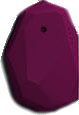
\includegraphics[scale=0.3]{../figures_chesta/diseno_del_exp/location_beacon.png}                                                                                                                  & 
\includegraphics[scale=0.3]{../figures_chesta/diseno_del_exp/proximity_beacon.png}                                                                                                                                                                                      & 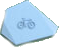
\includegraphics[scale=0.3]{../figures_chesta/diseno_del_exp/sticker_beacon.png}                                                                                                                                                                                                      & 
\includegraphics[scale=0.3]{../figures_chesta/diseno_del_exp/video_beacon.png}                                                                                                                                                                                                                \\
                                                                                        & \textbf{Locación}                                                                                                          & \textbf{Proximidad}                                                           & \textbf{Sticker}                                                                             & \textbf{Video}                                                                                        \\ \hline \hline
\multicolumn{1}{|c||}{\begin{tabular}[c]{@{}c@{}}\textbf{Vida útil}\\ \textbf{batería}\end{tabular}}       & Hasta 5 años                                                                                                            & Hasta 2 años                                                               & Hasta 1 año                                                                               & \begin{tabular}[c]{@{}c@{}}- \\ (conectado por USB)\end{tabular}                             \\ \hline
\multicolumn{1}{|c||}{\textbf{Rango}}                                                             & Hasta 200 metros                                                                                                        & Hasta 70 metros                                                            & Hasta 7 metros                                                                            & Hasta 10 metros                                                                                    \\ \hline
\multicolumn{1}{|c||}{\textbf{Grosor}}                                                            & 24 mm                                                                                                             & 17 mm                                                                & 6 mm                                                                                & 14 mm                                                                                        \\ \hline
\multicolumn{1}{|c||}{\begin{tabular}[c]{@{}c@{}}\textbf{Dispositivos}\\ \textbf{en el kit}\end{tabular}}  & 3 beacons                                                                                                         & 3 beacons                                                            & 10 stickers                                                                         & 3 mirrors                                                                                    \\ \hline
\multicolumn{1}{|c||}{\textbf{Precio}}                                                            & USD\$99                                                                                                           & USD\$59                                                              & USD\$99                                                                             & USD\$99                                                                                      \\ \hline
\end{tabular}
}
\end{table}

\begin{itemize}
\pause
\item \textit{Plug \& Play}
\pause
\item Baterías de litio 3[V] - 620[mAh]
\begin{itemize}
\pause
\item Costo: CLP\$5.000 - CLP\$6.000
\pause
\item Costo energético mensual: CLP\$250
\end{itemize}
\end{itemize}

\end{frame}

%------------------------------------------------

\begin{frame}
\frametitle{Cualidades y costos de tecnologías - RFID}

\vspace*{-.5cm}
\begin{table}[H]
\centering
\label{tab:rfid}
\resizebox{\textwidth}{!}{
\begin{tabular}{|c||c|c|c|}
\hline
\textbf{Tipo}                  & LF                                                                                          & HF                                                                                                & UHF                                                                                                        \\ \hline \hline
\textbf{Frecuencia}            & 125 kHz                                                                                     & 13.5 MHz                                                                                          & 915 MHz                                                                                                    \\ \hline
\textbf{Alcance}               & \textless 2.0 m                                                                             & \textless 1.0 m                                                                                   & \textgreater 3.0 m                                                                                         \\ \hline
\textbf{Aplicaciones}          & \begin{tabular}[c]{@{}c@{}}Identificación \\ de animales, \\ control de acceso\end{tabular} & \begin{tabular}[c]{@{}c@{}}Monedero, \\ Pasaporte, Tarjeta BIP, \\ control de acceso\end{tabular} & \begin{tabular}[c]{@{}c@{}}Logística, Retail, \\ Caja, Pallet, \\ Identificación de vehículos\end{tabular} \\ \hline

\end{tabular}
}
\end{table}

\begin{itemize}
\pause
\item Precio: Desde USD\$568.50\only<2->{\footnote{https://www.atlasfridstore.com/}}
\begin{itemize}
\item Reader: Desde USD\$450
\item Antena (9m): USD\$79
\item Cable conexión: USD\$39 (2m) - USD\$114 (10m)
\item Tag RFID Pasivo: USD\$0.50 - USD\$2

\end{itemize}

\pause
\item Consumo promedio mensual: 9[kWh]
\begin{itemize}
\pause
\item energético mensual: CLP\$1.011
\end{itemize}
\end{itemize}

\end{frame}

%------------------------------------------------

\begin{frame}
\frametitle{Cualidades y costos de tecnologías - Resumen}

\begin{table}[H]
\centering
\resizebox{\textwidth}{!}{
\begin{tabular}{|c|c|c|c|}
\hline
\textbf{Tecnología} & \begin{tabular}[c]{@{}c@{}}\textbf{Rango por} \\ \textbf{dispositivo}\end{tabular}& \textbf{Costo unitario}     & \begin{tabular}[c]{@{}c@{}}\textbf{Costo mensual} \\ \textbf{unitario}\end{tabular}\\ \hline 
\hline
Wi-Fi      & \begin{tabular}[c]{@{}c@{}}50 metros (802.11g) a \\ 70 metros (802.11n)\end{tabular} & Desde CLP\$17.990  & CLP\$607               \\ 
[3ex]\hline
Bluetooth  & 70-200 metros         & Desde CLP\$13.223\footnotemark[5]  & CLP\$250               \\ [3ex]\hline
RFID       & Desde 5 metros        & Desde CLP\$382.242\footnotemark[5] & CLP\$1.011             \\ [3ex]\hline
\end{tabular}
}
\end{table}

\footnotetext[5]{Dólar observado el 02/07/2017: CLP\$672,37. \\Fuente: Banco Central de Chile.}

\end{frame}

%------------------------------------------------
\subsection{Lugar del estudio}

\begin{frame}
\frametitle{Lugar del estudio}

\begin{figure}
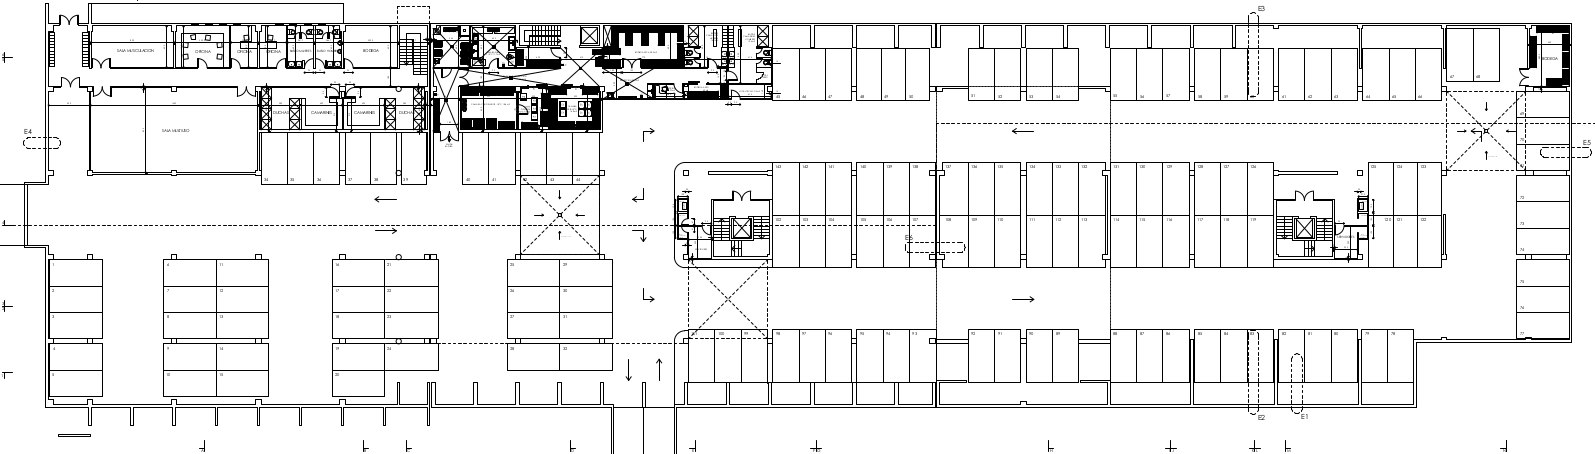
\includegraphics[width=\textwidth]{../figures_chesta/diseno_del_exp/plano_est}
\end{figure}

Estacionamiento subterráneo del Campus San Joaquín - Universidad Técnica Federico Santa María

\end{frame}

%------------------------------------------------
\begin{comment}
\subsection{Diseño de la Aplicación}

\begin{frame}
\frametitle{Diseño de la Aplicación}

\begin{itemize}

\item Aplicación móvil en Android

\item Requerimientos:
\begin{enumerate}[1]
\item Mostrar el plano de la ubicación
\item Permitir al usuario colocar marcadores de dispositivos Beacon/Access Point
\item Calcular la posición del usuario
\item Permitir al usuario agregar un marcador de la ubicación real
\item Calcular la distancia entre ubicación real y la calculada
\item Registrar las distancias en un archivo persistente
\end{enumerate}

\end{itemize}

\end{frame}
\end{comment}

%------------------------------------------------
\section{Implementación}
%------------------------------------------------

\subsection{Requerimientos}
\begin{frame}
\frametitle{Requerimientos}

\begin{enumerate}[1]
\pause
\item Mostrar el plano de la ubicación
\pause
\item Permitir al usuario colocar marcadores de dispositivos Beacon/Access Point
\pause
\item Calcular la posición del usuario
\pause
\item Permitir al usuario agregar un marcador de la ubicación real
\pause
\item Calcular la distancia entre ubicación real y la calculada
\pause
\item Registrar las distancias en un archivo persistente
\end{enumerate}


\end{frame}

%------------------------------------------------

\subsection{Ejecución}
\begin{frame}
\frametitle{Ejecución}

\begin{columns}

\column{.7\textwidth}

\begin{itemize}

\item Áreas de medición: \\7,95$[m^2]$ - 25,09$[m^2]$ - 27,64$[m^2]$ - 84,52$[m^2]$ - 118,37$[m^2]$
\visible<2->{
\item 200 mediciones por área}
\visible<3->{
\item Usuario inmóvil}
\visible<4->{
\item Método de mitigación: \textit{ventana deslizante}}

\end{itemize}


\column{.3\textwidth}

\begin{figure}
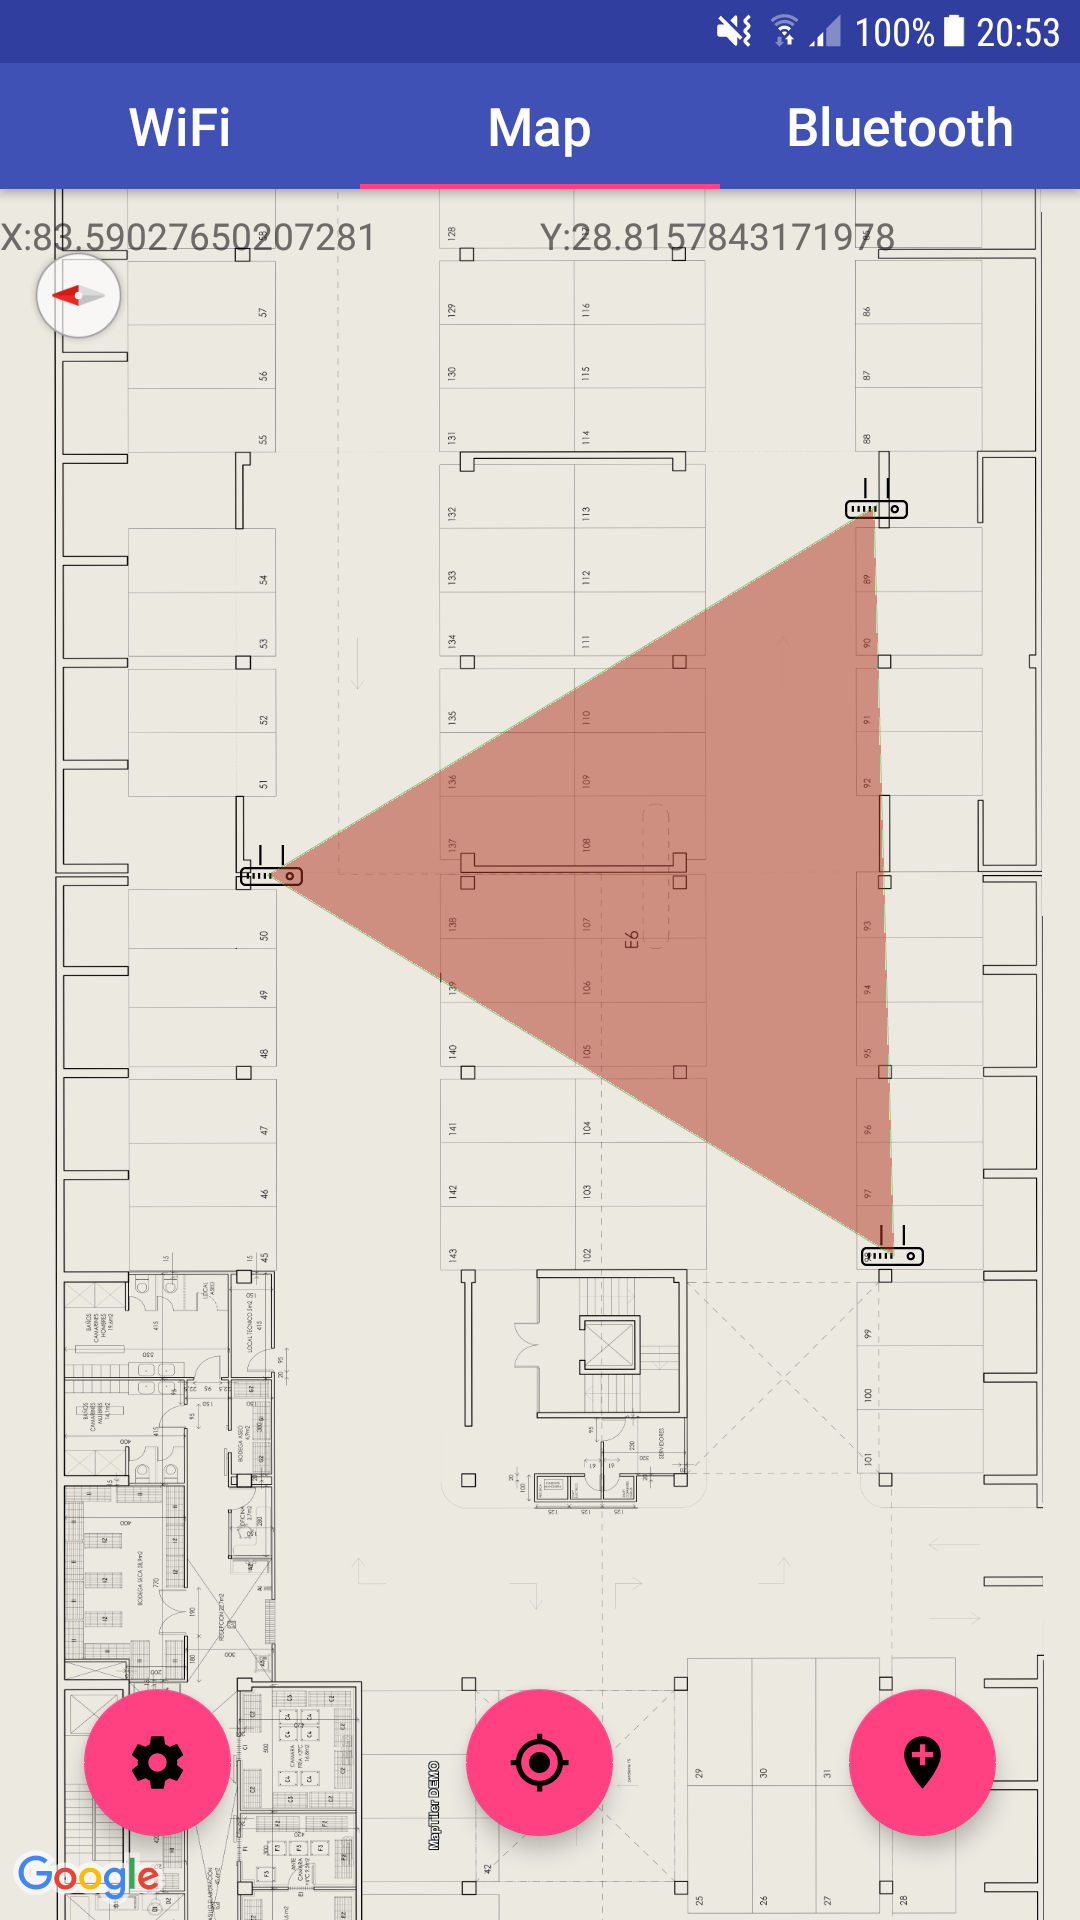
\includegraphics[width=\textwidth]{../figures_chesta/implementacion/triangle_area}
\end{figure}

\end{columns}

\end{frame}


%------------------------------------------------
\section{Resultados}
%------------------------------------------------

\begin{frame}
\frametitle{Área 7,95$[m^2]$}

\textbf{Posiciones calculadas}

\begin{figure}
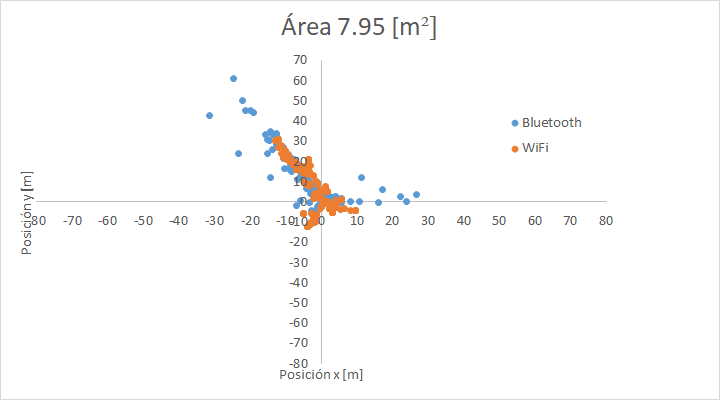
\includegraphics[width=\textwidth]{../figures_chesta/resultados/posicion__7_95}
\end{figure}


\end{frame}

%------------------------------------------------

\begin{frame}
\frametitle{Área 7,95$[m^2]$}

\textbf{Errores entre posición real y calculada}

\begin{figure}
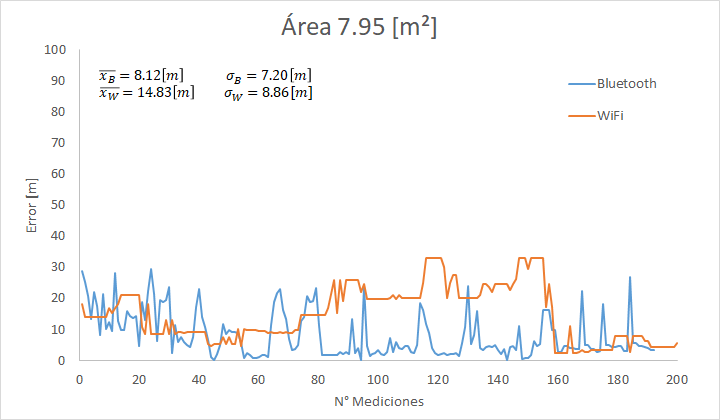
\includegraphics[width=\textwidth]{../figures_chesta/resultados/area__7_95}
\end{figure}



\end{frame}

%------------------------------------------------

\begin{frame}
\frametitle{Área 25,09$[m^2]$}

\textbf{Posiciones calculadas}

\begin{figure}
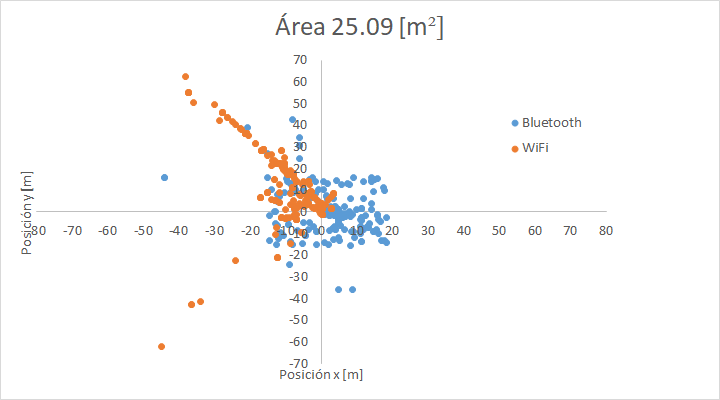
\includegraphics[width=\textwidth]{../figures_chesta/resultados/posicion__25_09}
\end{figure}


\end{frame}

%------------------------------------------------

\begin{frame}
\frametitle{Área 25,09$[m^2]$}

\textbf{Errores entre posición real y calculada}

\begin{figure}
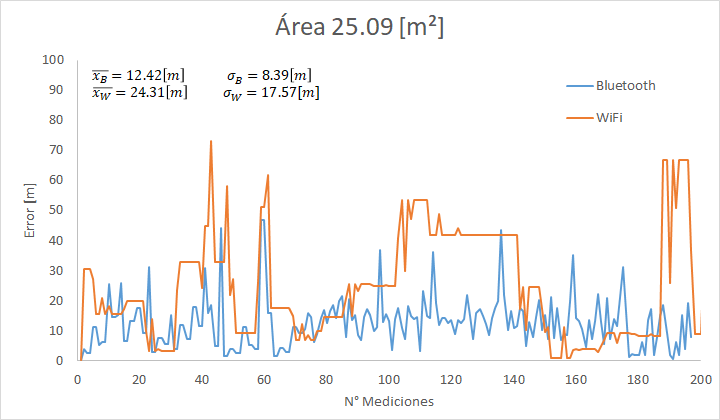
\includegraphics[width=\textwidth]{../figures_chesta/resultados/area__25_09}
\end{figure}



\end{frame}

%------------------------------------------------

\begin{frame}
\frametitle{Área 27,64$[m^2]$}

\textbf{Posiciones calculadas}

\begin{figure}
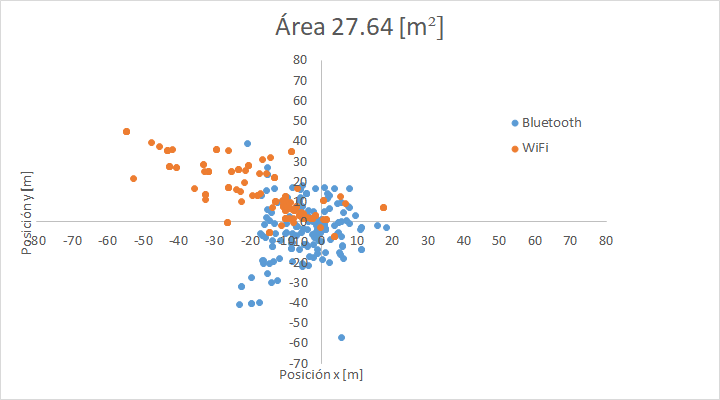
\includegraphics[width=\textwidth]{../figures_chesta/resultados/posicion__27_64}
\end{figure}


\end{frame}

%------------------------------------------------

\begin{frame}
\frametitle{Área 27,64$[m^2]$}

\textbf{Errores entre posición real y calculada}

\begin{figure}
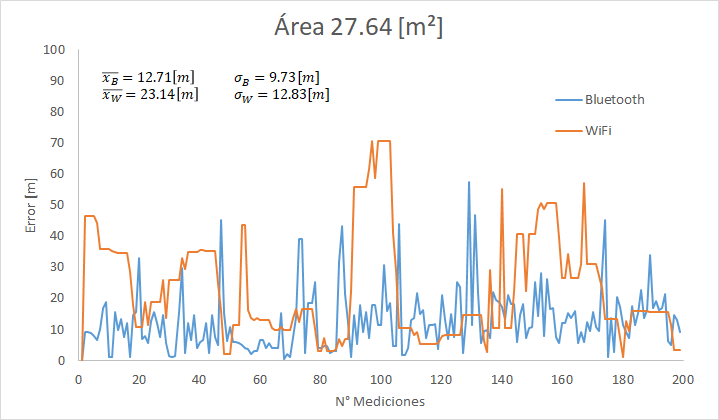
\includegraphics[width=\textwidth]{../figures_chesta/resultados/area__27_64}
\end{figure}



\end{frame}

%------------------------------------------------

\begin{frame}
\frametitle{Área 84,52$[m^2]$}

\textbf{Posiciones calculadas}

\begin{figure}
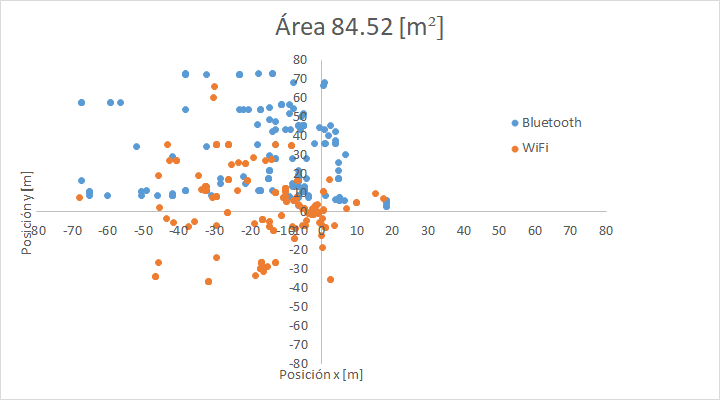
\includegraphics[width=\textwidth]{../figures_chesta/resultados/posicion__84_52}
\end{figure}


\end{frame}

%------------------------------------------------

\begin{frame}
\frametitle{Área 84,52$[m^2]$}

\textbf{Errores entre posición real y calculada}

\begin{figure}
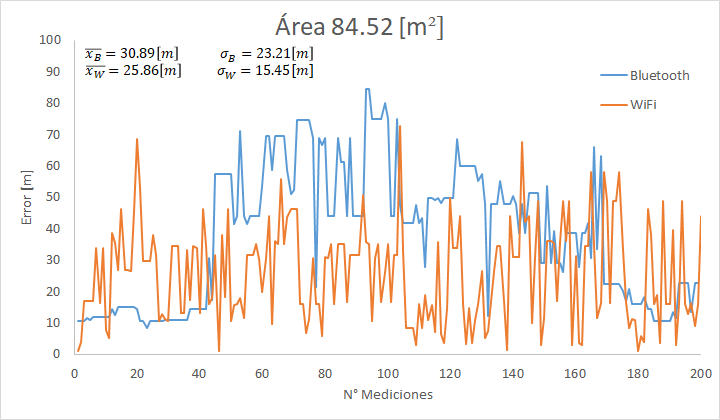
\includegraphics[width=\textwidth]{../figures_chesta/resultados/area__84_52}
\end{figure}



\end{frame}

%------------------------------------------------

\begin{frame}
\frametitle{Área 118,37$[m^2]$}

\textbf{Posiciones calculadas}

\begin{figure}
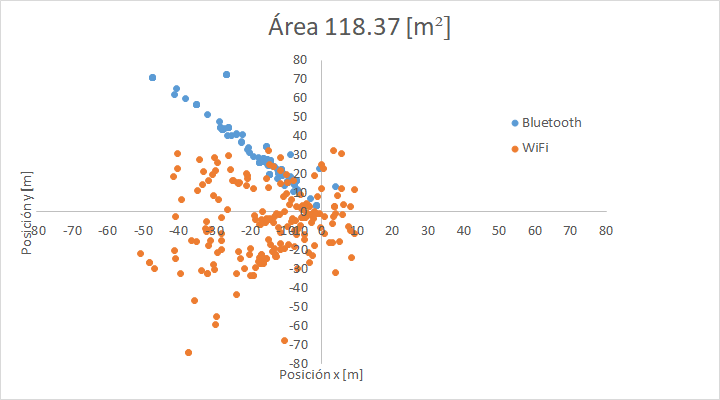
\includegraphics[width=\textwidth]{../figures_chesta/resultados/posicion__118_37}
\end{figure}


\end{frame}

%------------------------------------------------

\begin{frame}
\frametitle{Área 118,37$[m^2]$}

\textbf{Errores entre posición real y calculada}

\begin{figure}
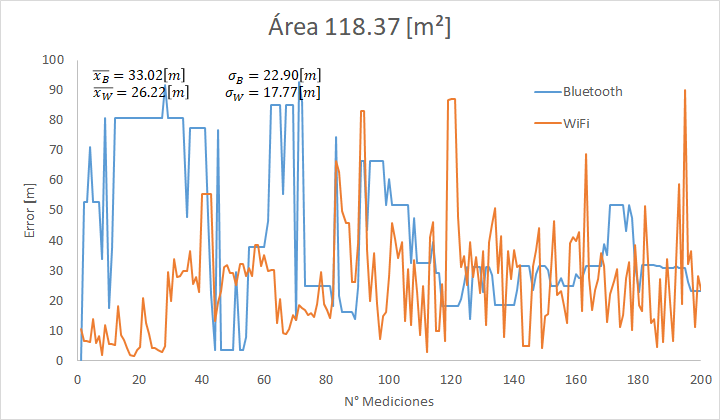
\includegraphics[width=\textwidth]{../figures_chesta/resultados/area__118_37}
\end{figure}



\end{frame}

%------------------------------------------------

\begin{frame}
\frametitle{Resumen resultados}

\begin{figure}
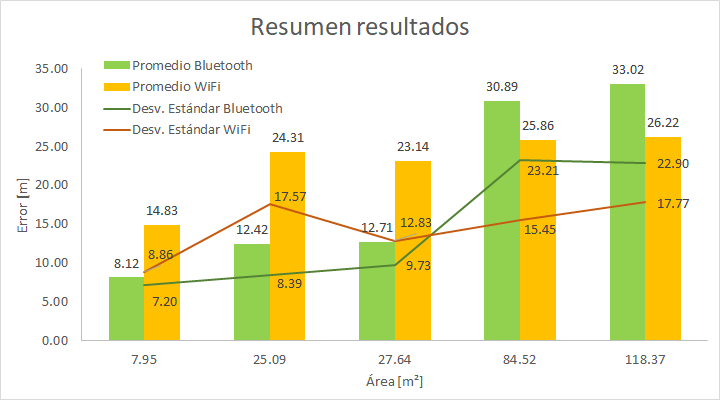
\includegraphics[width=\textwidth]{../figures_chesta/resultados/summary}
\end{figure}


%\begin{table}[H]
%\centering
%\label{tab:resumen_resultados}
%\resizebox{53.5ex}{!}{
%\begin{tabular}{ccccccc}
%\hline
%\textbf{Área {[}$m^2${]}}         & \multicolumn{2}{c}{7,95} & \multicolumn{2}{c}{25,09} & \multicolumn{2}{c}{27,64} \\ \hline
%\textbf{Tecnología}               & Bluetooth     & WiFi      & Bluetooth      & WiFi      & Bluetooth      & WiFi\\ \hline
%\textbf{Promedio [m]}      & 8,12          & 14,83     & 12,42          & 24,31     & 12,71          & 23,14     \\ \hline
%\textbf{Desv. estándar [m]} & 7,20          & 8,86      & 8,39           & 17,57     & 9,73           & 12,83\\ \hline
%\end{tabular}
%}
%\end{table}

%\begin{table}[H]
%\centering
%\label{tab:resumen_resultados}
%\resizebox{43ex}{!}{
%\begin{tabular}{ccccc}
%\hline
%\textbf{Área {[}$m^2${]} }        & \multicolumn{2}{c}{84,52} & \multicolumn{2}{c}{118,37} \\  \hline
%\textbf{Tecnología}               &  Bluetooth      & WiFi      & Bluetooth      & WiFi       \\ \hline
%\textbf{Promedio [m]}     &  30,89          & 25,86     & 33,02          & 26,22      \\ \hline
%\textbf{Desv. estándar [m]} &  23,21          & 15,45     & 22,90          & 17,77      \\ %\hline
%\end{tabular}
%}
%\end{table}

\end{frame}

%------------------------------------------------
\section{Conclusiones}
%------------------------------------------------

\begin{frame}
\frametitle{Conclusiones}

\begin{itemize}
\item Para áreas reducidas, Bluetooth es más efectivo que WiFi
\pause
\item Para áreas mayores, WiFi presenta un error más estable
\pause
\item La precisión y exactitud del posicionamiento depende de la densidad de dispositivos
\pause
\item Importancia en algoritmos de localización
\pause
%\item Numerosa presencia de señales inalámbricas
%\pause
\item El posicionamiento indoor aún es un campo abierto de estudio

\end{itemize}

\end{frame}

%------------------------------------------------

\begin{frame}
\Huge{\centerline{Gracias por su atención}}
\end{frame}

%------------------------------------------------

\end{document}
